% tikz/figure1.tex
\documentclass[tikz,border=10pt]{standalone}
\usepackage{tikz}
\usepackage{contour}
\usepackage{readarray}
% any other packages you need

\begin{document}
\centering
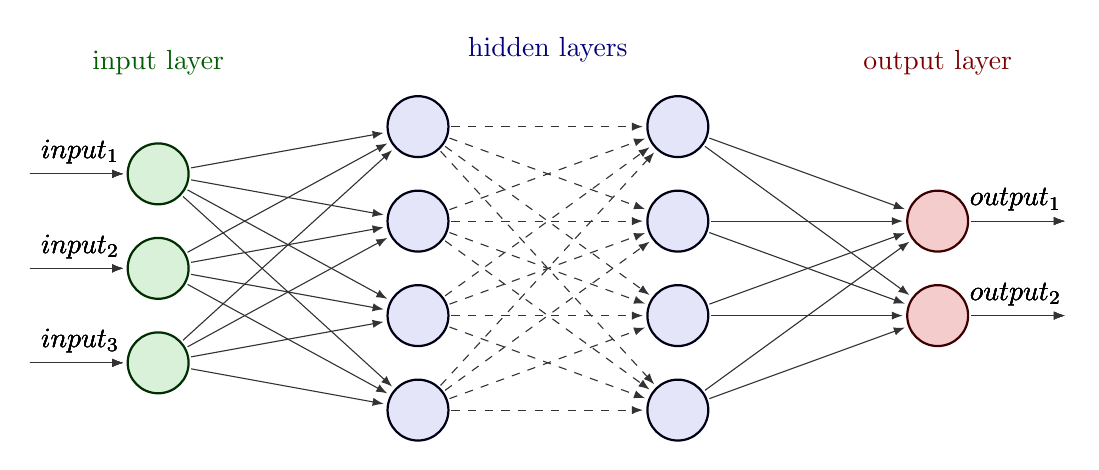
\begin{tikzpicture}[x=3.3cm,y=1.2cm]
\usetikzlibrary{arrows.meta} % for arrow size
\usetikzlibrary{calc}
\contourlength{1.4pt}
\colorlet{myred}{red!80!black}
\colorlet{myblue}{blue!80!black}
\colorlet{mygreen}{green!60!black}
\colorlet{myorange}{orange!70!red!60!black}
\colorlet{mydarkred}{red!30!black}
\colorlet{mydarkblue}{blue!40!black}
\colorlet{mydarkblack}{gray!40!black}

\colorlet{mydarkgreen}{green!30!black}
\tikzset{
  >=latex, % for default LaTeX arrow head
  node/.style={thick,circle,draw=myblue,minimum size=22,inner sep=0.5,outer sep=0.6},
  node in/.style={node,green!20!black,draw=mygreen!30!black,fill=mygreen!15},
  node hidden/.style={node,blue!10!black,draw=myblue!10!black,fill=myblue!10},
  node convol/.style={node,orange!20!black,draw=myorange!30!black,fill=myorange!10},
  node out/.style={node,red!20!black,draw=myred!30!black,fill=myred!20},
  connect/.style={mydarkblack}, %,line cap=round
  connect arrow/.style={-{Latex[length=4,width=3]},mydarkblack,shorten <=0.5,shorten >=1},
  node 1/.style={node in}, % node styles, numbered for easy mapping with \nstyle
  node 2/.style={node hidden},
  node 3/.style={node out}
}
\def\nstyle{int(\lay<\Nnodlen?min(2,\lay):3)} % map layer number onto 1, 2, or 3
  \message{^^JNeural network without text}
  \readlist\Nnod{3,4,4,2} % array of number of nodes per layer
  
  \message{^^J  Layer}
  \foreachitem \N \in \Nnod{ % loop over layers
    \def\lay{\Ncnt} % alias of index of current layer
    \pgfmathsetmacro\prev{int(\Ncnt-1)} % number of previous layer
    \message{\lay,}
    \foreach \i [evaluate={\y=\N/2-\i; \x=\lay; \n=\nstyle;}] in {1,...,\N}{ % loop over nodes
      
      % NODES
      \node[node \n] (N\lay-\i) at (\x,\y) {};
      
      % CONNECTIONS
      \ifnum\lay>1 % connect to previous layer
        \foreach \j in {1,...,\Nnod[\prev]}{ % loop over nodes in previous layer
            \ifnum\prev>1
                \ifnum\lay<\Nnodlen
                    \draw[connect arrow,dashed] (N\prev-\j) -- (N\lay-\i);
                \else
                    \draw[connect arrow] (N\prev-\j) -- (N\lay-\i);
                \fi
            \else
                \draw[connect arrow] (N\prev-\j) -- (N\lay-\i);
            \fi          %\draw[connect] (N\prev-\j.0) -- (N\lay-\i.180); % connect to left
            
            \ifnum\prev=1
                \draw[connect arrow] ($(N\prev-\j) - (0.5,0)$) -- (N\prev-\j);
                \node[anchor=south] at ($(N\prev-\j) - (0.3,0)$) {$input_\j$};
            \fi

            \ifnum\lay=\Nnodlen
                \draw[connect arrow] (N\lay-\i) -- ($(N\lay-\i) + (0.5,0)$);
                \node[anchor=south] at ($(N\lay-\i) + (0.3,0)$) {$output_\i$};

            \fi
            
        }
      \fi % else: nothing to connect first layer
      
    }
  }
  
  % LABELS
  \node[above=15,align=center,mygreen!60!black,font=\normalfont] at ($(N2-1)-(1,0)$) {input layer};
\node[above=20,align=center,myblue!60!black,font=\normalfont] at ($(N2-1)!0.5!(N3-1)$) {hidden layers};
\node[above=15,align=center,myred!60!black,font=\normalfont] at ($(N3-1)+(1,0)$) {output layer};

  %\node[above=15,align=center,mygreen!60!black] at ($(N2-1) - (1, 0)$) {input layer};
  %\node[above=20,align=center,myblue!60!black] at ($(N2-1)!0.5!(N3-1)$) {hidden layers};
  %\node[above=15,align=center,myred!60!black] at ($(N3-1) + (1, 0)$) {output layer};
  
\end{tikzpicture}
% your TikZ code here
\end{document}